\documentclass[]{article}

\usepackage[pdftex]{graphicx}
\usepackage[top=1in, bottom=1in, right=1.25in, left=1.25in]{geometry}
\usepackage{hyperref}
\usepackage{pdfpages}

\begin{document}

	% Title Page
	\begin{titlepage}



		\title{\textbf{Review of Technical Specifications}}
		\author{BU ProPane Team:\\Griffin Dunn\\Colin Madigan\\Phillip Stahlfeld}
		\date{April 15, 2013}
		\maketitle



		\noindent
		
		\thispagestyle{empty}

	\end{titlepage}
	
	\thispagestyle{empty}
	
	
	% Begin  Real  Document
	%\tableofcontents
	%\newpage
	
	
	\setcounter{page}{1}
	\thispagestyle{empty}
	
	\section*{Specification Overview}
		The following table shows an overview of the technical specifications for this project. A larger version of this table has been provided on the last page. The important thing to note about this table is that all of the required specifications have been met (green) in addition to one additional feature (blue).\\
		\begin{figure}[h!]
			\centering
			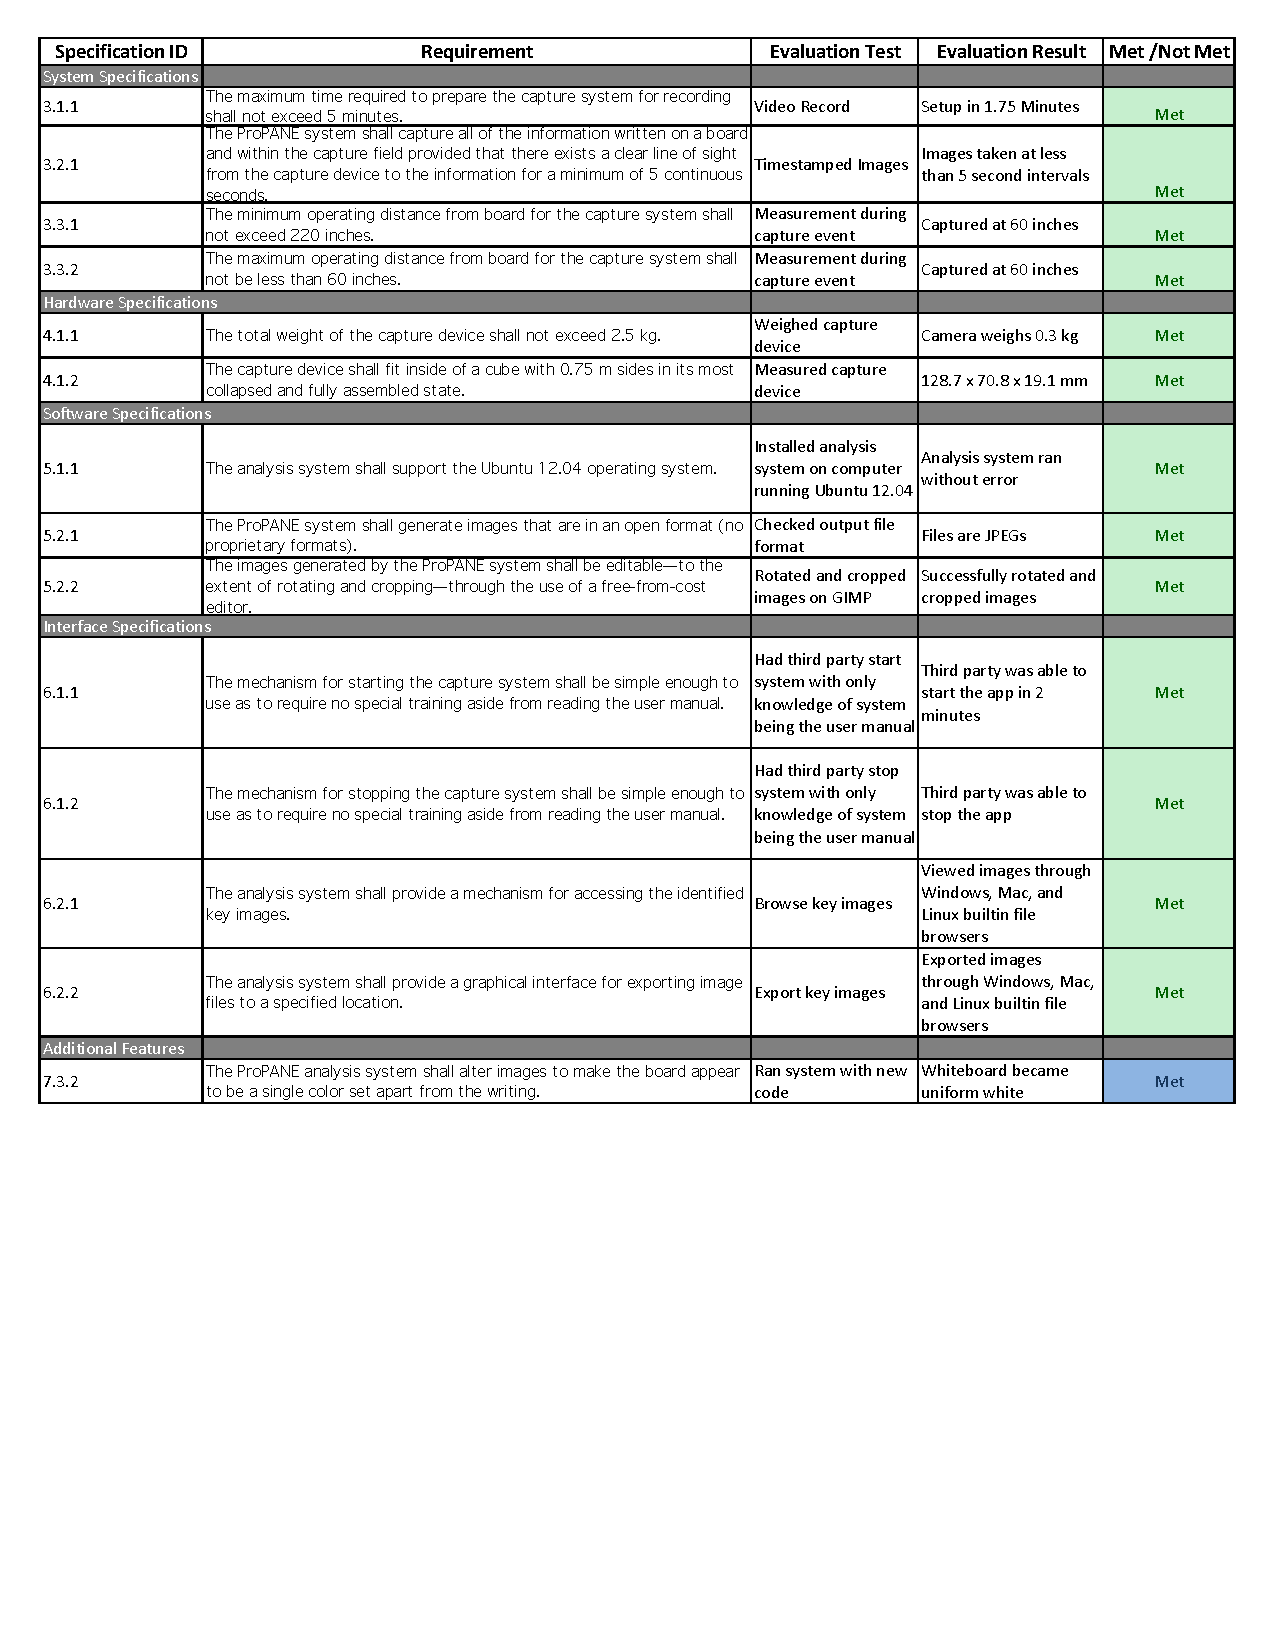
\includegraphics[scale=0.5]{technicalspecificationreview.pdf}
		\end{figure}
		
	\section*{Specification Changes}
		The only specification that has been altered since the beginning of the year is 5.1.1 where the operating system to be supported was originally 10.04. This minor change was approved by our clients. 
		
	\section*{Additional Specifications}
		It seems like a lot of the specifications for this project relate to the usage of the system and not quantifiable measures of what the system will actually have to accomplish. Even with the knowledge acquired from the process of creating this system, we still find it difficult to create specifications for the system while still keeping it implementation agnostic. However, if we did this project again, we would add the following specifications for how the system should function:
		\begin{itemize}
			\item A key image shall be generated when at least 5\% of all writing on the board and within the capture field has changed or been erased.
			\item The system shall be capable of capturing all information written on a board with dimensions 6 feet by 4 feet.
		\end{itemize}
		The first requirement would be used to ensure that the system is actually generating key images correctly. The second requirement would be used to ensure that the system is actually capturing a usable amount of board space.
		
		
	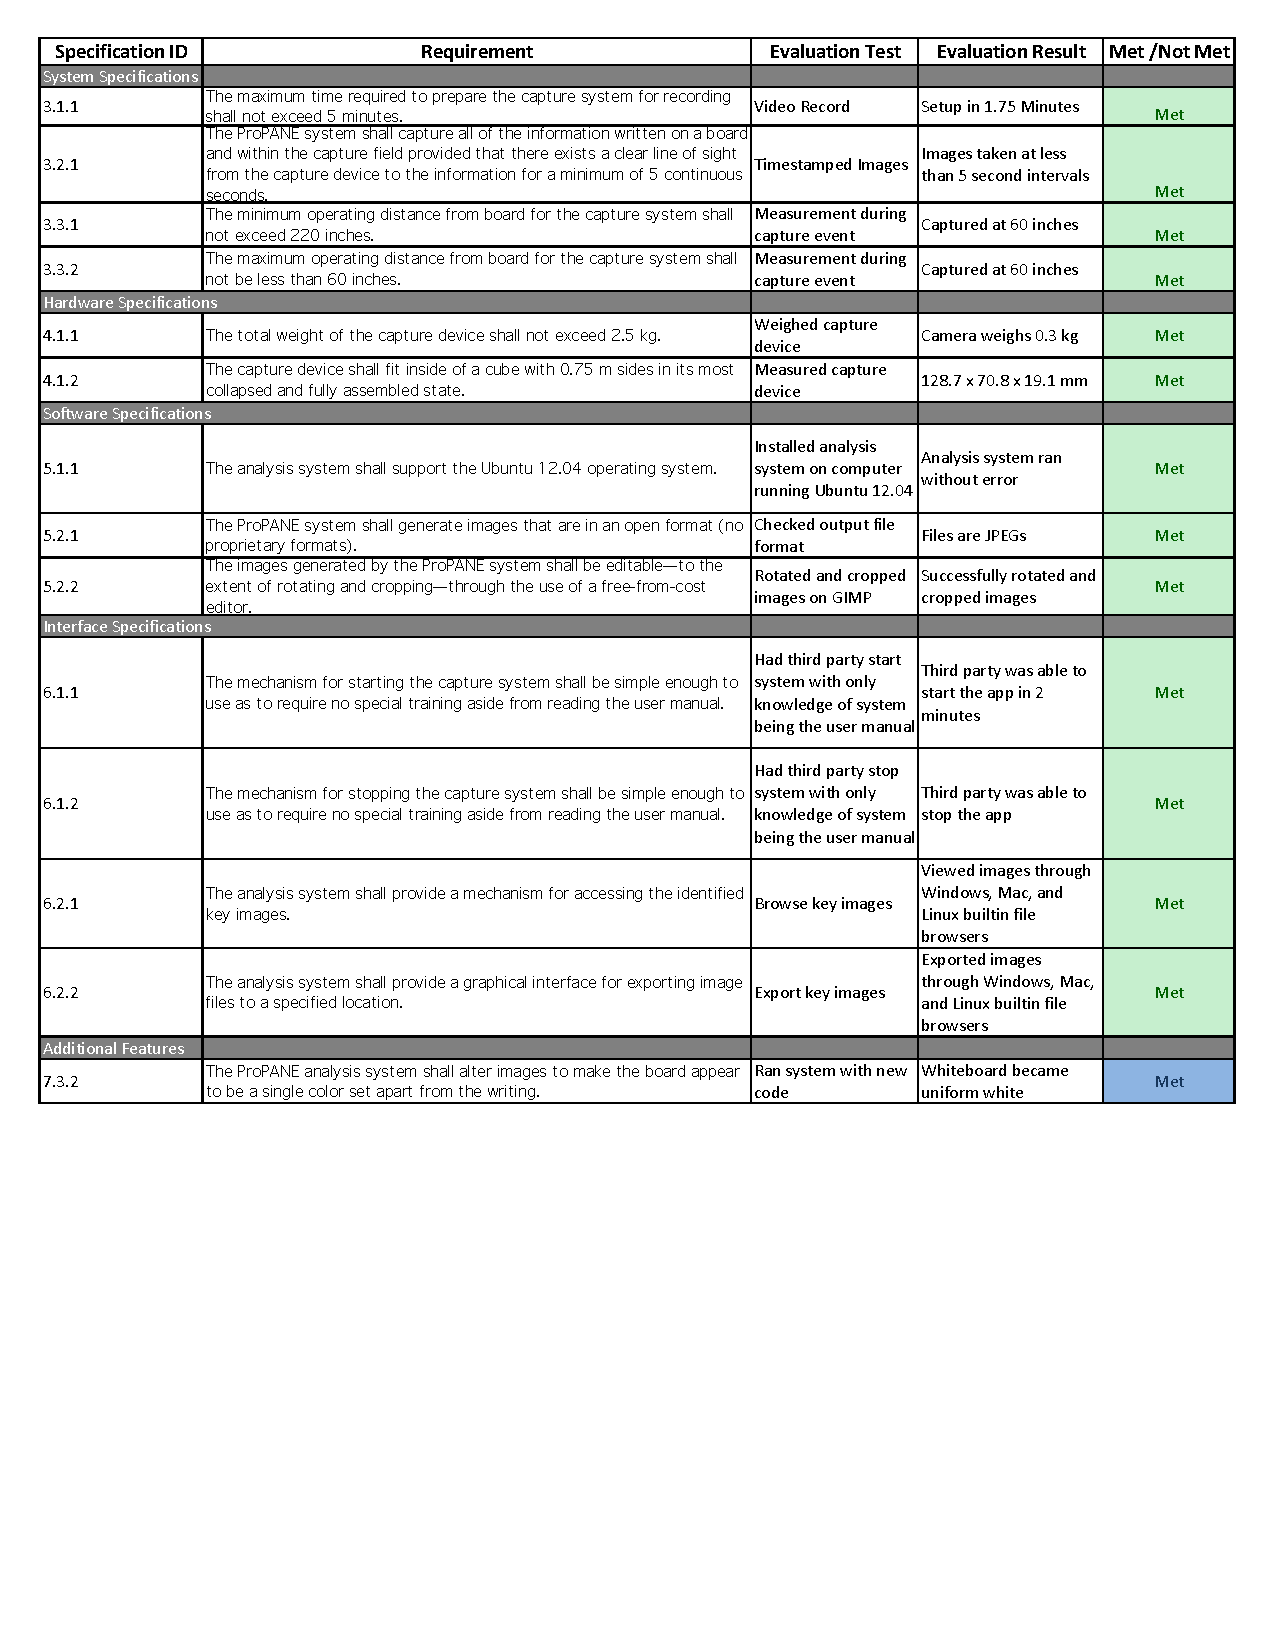
\includepdf{technicalspecificationreview.pdf}
	
\end{document}